\section{Literate Programming}
\label{sec:literate-programming}
Just as with REPLs, the concept of literate programming is implemented in
various forms under various names. Therefore this section starts with an
explanation of what literate programming is exactly based on a few
implementations. Afterwards, the IPython implemention of literate programming is
explored in more detail.

Literate programming, as defined in~\cite{knuth1984}, introduces the ability to
annotate source code with natural language. According to Donald Knuth, better
documentation of programs is essential to make further progress in the state of
the art of programming.  To achieve this he proposes to write programs not with
the intention to explain the computer what to do, but with the intention to
explain to humans what the programmer wants a computer to do~\cite{knuth1984},
by mixing documentation and source code in a single file. This idea of
literate programming was realized in its original form as the ``WEB'' language
developed during Knuth's research at Stanford University.

Even though the idea was conceived over 30 years ago, implementations are not
very common. However, in recent years the idea seems to gain popularity again.
A very recent implementation of literate programming is Apple's Swift
playgrounds~\cite{swift-playgrounds}. Swift playgrounds are interactive
documents or ``notebooks'' in which code is executed as it is typed, in
contrast to the non-interactive style of ``WEB'' language in which \TeX{} and
PASCAL were combined into one language: \TeX{} served to describe the program
and PASCAL to produce a machine-executable program.

In recent years, there has also been a particular focus on reproducible
research. While literate programming primarily aims to add documentation to
code, reproducible research focuses on adding code to documentation. More
specifically, reproducible research refers to the idea that scientific papers
should be augmented with the computer code used to carry out the
research~\cite{schulte2012}. Examples of recent projects claiming to support
both reproducible research and literate programming include the IPython
project~\cite{ipython2007} and Emacs Org-mode~\cite{schulte2012}.

\subsubsection{IPython with Jupyter notebooks}

As explained in the introduction, IPython (together with Jupyter notebooks)
supports both reproducible research and literate programming. IPython was
partially inspired by other scientific tools already offering notebook-like
functionality, such as Matlab or Mathematica. Since its inception, the project
has been split off into IPython, which provides an interactive REPL and a
kernel that runs the user's code, and Jupyter notebooks, which provide the
notebook format and web application. Like Swift playgrounds, Jupyter notebooks
allow for REPL-style interactive editing; documentation and code can be edited
live and blocks of code can be reevaluated, printing their updated results.
Jupyter notebooks also allow for more complex graphical elements such as
3D-plots. See \cref{fig:ipython} for an example of an IPython notebook.

\begin{figure}[htb]
  \centering
  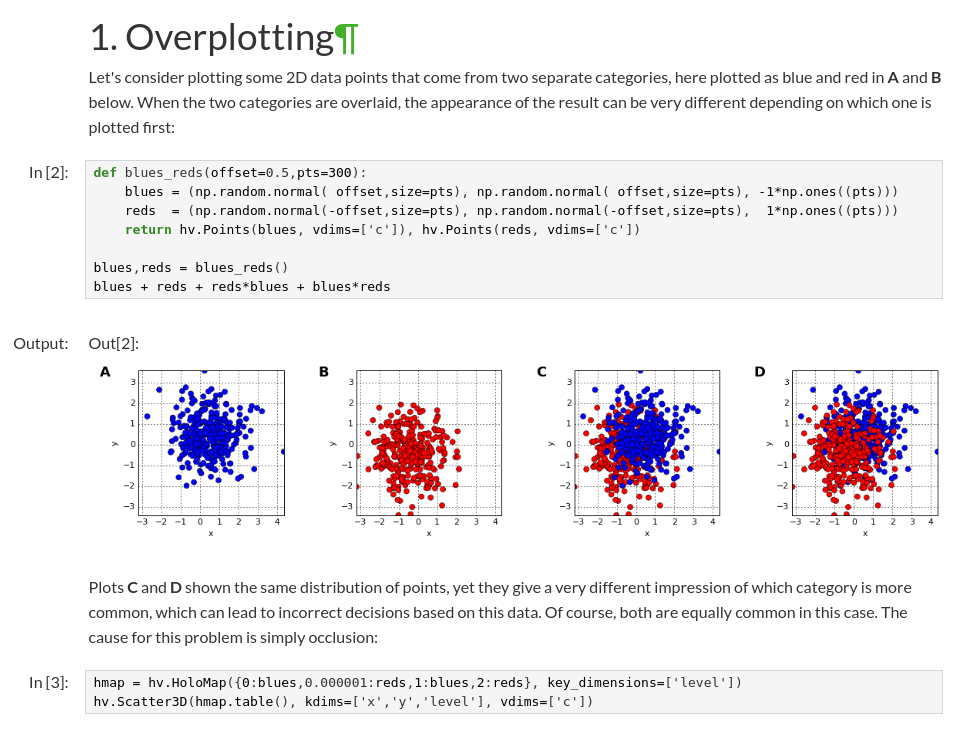
\includegraphics[width=\textwidth]{ipython}
  \caption{A plot from data in an IPython notebook.}
  \label{fig:ipython}
\end{figure}

As explained, IPython and Jupyter notebooks have become more or less separate
projects, to the extent that Jupyter notebooks can use several kernels.
Nowadays there are kernels for over 40 languages that can be used in these
notebooks. This illustrates that in Python's case literate programming is more
or less an extension to the interactive IPython REPL. Since Jupyter notebooks
reuse the IPython REPL, the execution model used for Jupyter notebooks is
essentially the same as it is for IPython~\cite{ipython-execution}.

%%% Local Variables:
%%% mode: latex
%%% TeX-master: "main"
%%% End:
